\documentclass[12pt,a4paper]{article}

% Margins.
\setlength{\oddsidemargin}{0in}
\setlength{\evensidemargin}{0in}
\setlength{\headheight}{12pt}
\setlength{\headsep}{42pt}
\setlength{\topmargin}{-54pt}
\setlength{\textwidth}{6.5in}
\setlength{\textheight}{10in}

\usepackage{amsmath}
\usepackage{float}
\usepackage{graphicx}
\usepackage[hyphens]{url}
\usepackage{hyperref}	% Clickable links to figures, references and urls.

% Drawing.
\usepackage{pgf}
\usepackage{tikz}
\usepackage{amssymb}  % Tick mark
\usepackage{textcomp} % Cross

% Listings for formatting code.
\usepackage{listings}
\usepackage{textcomp}
% General options.
\lstset{breaklines=true, basicstyle=\small\ttfamily, tabsize=4, numbers=left, stepnumber=1, frame=single, showstringspaces=false, upquote=true}
% C++ specific high-lighting. Comments are 50/50 shades of green/black and strings coloured with 60/40 red/black mixture.
\lstset{language=[ISO]C++, commentstyle=\color{green!50!black}, keywordstyle=\color{blue}, stringstyle=\color{red!60!black}}

%opening
\title{\vspace{-2cm}Programming for Engineers I\\Class 18\\C--Strings}
\author{Attique Dawood}

\begin{document}
\maketitle
\section{Announcements}
\begin{itemize}
\item Quiz \# 4 on Friday 15-03-2013.
\end{itemize}
\section{Revision}
\begin{itemize}
\item Functions.
\end{itemize}
\section{C--Strings}
\begin{itemize}
\item C--strings are char arrays.
\item Meaningful characters in C--strings are terminated with a NULL character (\verb|'\0'|).
\end{itemize}
\section{What are C--Strings?}
Simple answer: character arrays are called C--string or `string' for short. A bunch of characters most often only make sense if they form words. And words only make sense if they are part of a sentence. Essentially, character arrays are used for storage of words, sentences or the like.
\section{Initialization at Declaration}
Character arrays have an additional way of initialisation, in addition to other array initialisation methods. Without specifying size, a char array is assigned a string at declaration. In this case, compiler automatically allocates space for array.
\begin{lstlisting}[caption={Initialisation of C--Strings}]
char myName1[] = "my name 1";  // Method 1.
char myName2[20] = "my name 2" // Method 2.
char myName3[20]; // Declaration.
strcpy(myName3, "My name 3"); // Using strcpy to initialise.
cout << myName1 << endl; // Display.
\end{lstlisting}
\section{The \texttt{NULL} Character}
You might ask the question, when using \texttt{cout} how does the compiler know when the string ends? The answer is that every string ends (or must end) with a \texttt{NULL} character (or \verb|'\0'| in ASCII). In above example, \texttt{myName1} was allocated 4 bytes by compiler to end the string with a \verb|'\0'| character. Built-in string functions like this one automatically append \verb|'\0'| at the end of a string. In case you are working or manipulating character arrays directly, then you must take care of \verb|'\0'| yourself.
\section{Length of String}
Length of a string does not include \verb|'\0'|. It only counts the total number of characters before \verb|'\0'|. The \textbf{size of array} containing string and \textbf{length of string} are two different things. In the code segment below, size of array is 10 and length of stored string is 3.
\begin{lstlisting}
char myName[10];
myName[0] = 'a';
myName[1] = 'b';
myName[2] = 'c';
myName[3] = '\0'; // Terminating NULL character.
cout << myName << endl;
Output:
abc
\end{lstlisting}
\section{String Input}
Strings can be input using either \texttt{cin} or \texttt{cin.getline()} functions. \texttt{cin} cannot input spaces so \texttt{getline} should be used if input string contains spaces. \verb|cin.getline()| copies a NULL in the last index. Size passed in \verb|cin.getline()| function should be equal to the array size. In the following code it will be ensured by \verb|cin.getline()| that 20th character is NULL if input exceeds or is equal to 20 characters. If input is less than 20 characters then a NULL will be appended after last input character.
\begin{lstlisting}[caption={String input using cin.getline()}]
char myName[20];
cin.getline(myName, 20);
\end{lstlisting}
Care should be taken when entering strings. The total number of characters must not exceed the size of array. In addition maximum number of characters must be 1 less than array size for a terminating \verb|`\0'|.
\begin{lstlisting}[caption={String size and NULL}]
char CourseName1[10] = "Physics";
char CourseName2[10] = "Programming for Engineers I";
char CourseName3[10] = "Calculus I";

Output:
Physics                          // Correct input, string length=7.
Programming for Engineers I      // WRONG! Input exceeds size of array.
Calculus I                       // WRONG! No space for `\0', string length=10.
\end{lstlisting}
\begin{figure}[H]
\centering
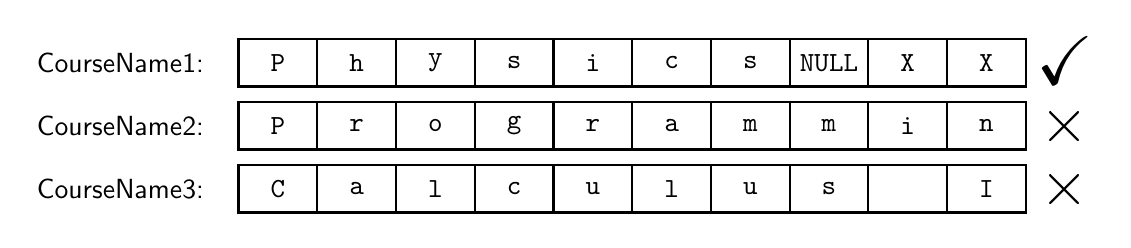
\begin{tikzpicture}
	\def \displacement {0.0cm}
	% Writing 'CourseName1'
	\draw (-1.5cm,\displacement+0.3cm) node {\textsf{CourseName1:}};
	% Drawing boxes.
	\foreach \x in {0.0cm, 1.0cm, 2.0cm, 3.0cm, 4.0cm, 5.0cm, 6.0cm, 7.0cm, 8.0cm, 9.0cm}
		\draw[thick] (\x, \displacement) rectangle (\x+1.0cm, \displacement+0.6cm);
	% Writing things in boxes.
	\foreach \x/\y in {0.0cm/P, 1.0cm/h, 2.0cm/y, 3.0cm/s, 4.0cm/i, 5.0cm/c, 6.0cm/s, 7.0cm/NULL, 8.0cm/X, 9.0cm/X}
		\draw (\x+0.5cm,\displacement+0.3cm) node {\texttt{\y}};
	% Tick.
	\coordinate [label=above:{\Huge \checkmark}] (Tick) at (10.5cm,\displacement-0.1cm);

	\def \displacement {-0.8cm}
	% Writing 'CourseName2'
	\draw (-1.5cm,\displacement+0.3cm) node {\textsf{CourseName2:}};
	% Drawing boxes.
	\foreach \x in {0.0cm, 1.0cm, 2.0cm, 3.0cm, 4.0cm, 5.0cm, 6.0cm, 7.0cm, 8.0cm, 9.0cm}
		\draw[thick] (\x, \displacement) rectangle (\x+1.0cm, \displacement+0.6cm);
	% Writing things in boxes.
	\foreach \x/\y in {0.0cm/P, 1.0cm/r, 2.0cm/o, 3.0cm/g, 4.0cm/r, 5.0cm/a, 6.0cm/m, 7.0cm/m, 8.0cm/i, 9.0cm/n}
		\draw (\x+0.5cm,\displacement+0.3cm) node {\texttt{\y}};
	% Cross.
	\coordinate [label=above:{\Huge \texttimes}] (Cross1) at (10.5cm,\displacement-0.1cm);

	\def \displacement {-1.6cm}
	% Writing 'CourseName3'
	\draw (-1.5cm,\displacement+0.3cm) node {\textsf{CourseName3:}};
	% Drawing boxes.
	\foreach \x in {0.0cm, 1.0cm, 2.0cm, 3.0cm, 4.0cm, 5.0cm, 6.0cm, 7.0cm, 8.0cm, 9.0cm}
		\draw[thick] (\x, \displacement) rectangle (\x+1.0cm, \displacement+0.6cm);
	% Writing things in boxes.
	\foreach \x/\y in {0.0cm/C, 1.0cm/a, 2.0cm/l, 3.0cm/c, 4.0cm/u, 5.0cm/l, 6.0cm/u, 7.0cm/s, 8.0cm/ , 9.0cm/I}
		\draw (\x+0.5cm,\displacement+0.3cm) node {\texttt{\y}};
	% Cross.
	\coordinate [label=above:{\Huge \texttimes}] (Cross2) at (10.5cm,\displacement-0.1cm);
\end{tikzpicture}
\end{figure}
\end{document}